\documentclass[./main.tex]{subfiles}

\begin{document}
\chapter{Analisi Sperimentale}
\section{La libreria TPTP}
\begin{figure}[h]
    \centering
    \scalebox{0.3}{
        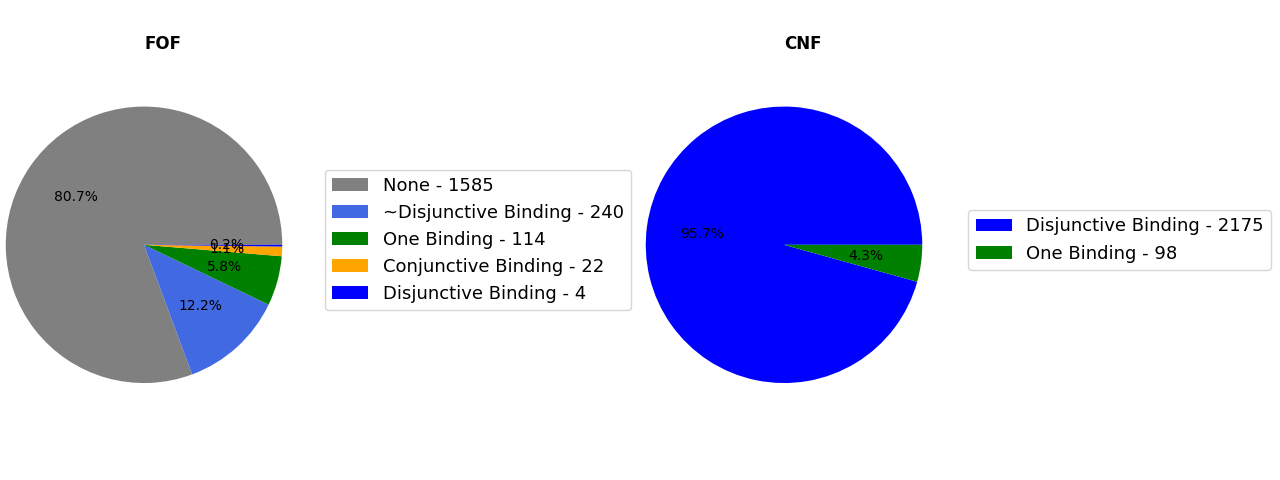
\includegraphics{images/5_sperimentazione/fof_cnf_classificazione.png}
    }
    \caption{Classificazione Libreria TPTP fof e cnf senza uguaglianza}
    \label{fig:classificazione_tptp}
\end{figure}
\section{Analisi dei risultati}
\begin{table}[H]
    \begin{minipage}{5cm}
        \resizebox{\textwidth}{!}{
            \begin{tabular}{|c|c|c|c|}
            \hline
            $N^\circ$ & Vampire & 1b naif & 1b \\
            \hline
            1 & 0.734 & 0.841 & 1.022 \\
            \hline
            2 & 0.567 & 0.814 & 0.521 \\
            \hline
            3 & 0.571 & 0.79 & 0.5 \\
            \hline
            4 & 0.603 & 0.786 & 0.591 \\
            \hline
            5 & 0.531 & 0.57 & 0.881 \\
            \hline
            6 & 0.625 & 0.402 & 0.354 \\
            \hline
            7 & 600000.0 & 600000.0 & 1.786 \\
            \hline
            8 & 0.788 & 0.647 & 0.358 \\
            \hline
            9 & 0.653 & 1.023 & 0.384 \\
            \hline
            10 & 0.691 & 1.039 & 0.366 \\
            \hline
            11 & 1.044 & 1.032 & 0.383 \\
            \hline
            12 & 0.592 & 0.489 & 0.323 \\
            \hline
            13 & 0.53 & 0.591 & 0.409 \\
            \hline
            14 & 0.602 & 0.395 & 0.451 \\
            \hline
            15 & 0.464 & 0.36 & 0.332 \\
            \hline
            16 & 0.734 & 0.364 & 0.335 \\
            \hline
            17 & 11.0 & 0.484 & 0.384 \\
            \hline
            18 & 0.974 & 0.585 & 0.359 \\
            \hline
            19 & 1.368 & 0.591 & 0.514 \\
            \hline
            20 & 1.292 & 0.571 & 0.396 \\
            \hline
            21 & 600000.0 & 5.353 & 1.044 \\
            \hline
            22 & 1.221 & 0.488 & 0.418 \\
            \hline
            23 & 342.0 & 6.848 & 1.1 \\
            \hline
            24 & 337.0 & 6.975 & 1.07 \\
            \hline
            25 & 600000.0 & 0.892 & 0.647 \\
            \hline
            26 & 242.0 & 0.806 & 0.584 \\
            \hline
            27 & 2.937 & 0.653 & 0.535 \\
            \hline
            28 & 39.0 & 1.93 & 1.071 \\
            \hline
            29 & 8.136 & 1.153 & 0.845 \\
            \hline
            30 & 3.402 & 1.036 & 0.684 \\
            \hline
            31 & 0.68 & 0.002852 & 0.002953 \\
            \hline
            32 & 0.645 & 0.002833 & 0.003199 \\
            \hline
            33 & 0.402 & 0.279 & 0.251 \\
            \hline
            34 & 0.229 & 0.248 & 0.224 \\
            \hline
            35 & 0.126 & 0 & 0 \\
            \hline
            36 & 0.398 & 0.281 & 0.249 \\
            \hline
            37 & 0.237 & 0.234 & 0.217 \\
            \hline
            38 & 18000.0 & 74.0 & 74.0 \\
            \hline
            39 & 34000.0 & 136.0 & 137.0 \\
            \hline
            \end{tabular}
        }
    \end{minipage}
    \begin{minipage}{5.02cm}
        \resizebox{\textwidth}{!}{    
\begin{tabular}{|c|c|c|c|}
\hline
$N^\circ$ & Vampire & 1b naif & 1b \\
\hline
40 & 598000.0 & 1.887 & 1.878 \\
\hline
41 & 584000.0 & 1.903 & 1.896 \\
\hline
42 & 598000.0 & 1.501 & 1.491 \\
\hline
43 & 598000.0 & 1.54 & 1.554 \\
\hline
44 & 598000.0 & 6.307 & 6.29 \\
\hline
45 & 0.614 & 0.003116 & 0.002933 \\
\hline
46 & 0.443 & 0.347 & 0.289 \\
\hline
47 & 0.44 & 0.002824 & 0.002807 \\
\hline
48 & 0.604 & 0.002817 & 0.002902 \\
\hline
49 & 0.465 & 0.002864 & 0.002794 \\
\hline
50 & 1.455 & 0.026 & 0.026 \\
\hline
51 & 3.638 & 0.032 & 0.033 \\
\hline
52 & 0.608 & 0.002861 & 0.00295 \\
\hline
53 & 600000.0 & 0.042 & 0.044 \\
\hline
54 & 2.662 & 0.595 & 0.441 \\
\hline
55 & 1.09 & 0.594 & 0.313 \\
\hline
56 & 1.188 & 0.936 & 0.48 \\
\hline
57 & 1.128 & 0.35 & 0.31 \\
\hline
58 & 0.953 & 0.385 & 0.311 \\
\hline
59 & 0.957 & 0.385 & 0.393 \\
\hline
60 & 0.691 & 0.474 & 0.294 \\
\hline
61 & 2.078 & 0.792 & 0.575 \\
\hline
62 & 0.443 & 0.358 & 0.298 \\
\hline
63 & 0.421 & 0.003014 & 0.002854 \\
\hline
64 & 0.429 & 0.002817 & 0.00294 \\
\hline
65 & 0.447 & 0.002823 & 0.003353 \\
\hline
66 & 0.458 & 0.002869 & 0.0031 \\
\hline
67 & 0.852 & 0.023 & 0.024 \\
\hline
68 & 600000.0 & 0.038 & 0.038 \\
\hline
69 & 600000.0 & 0.07 & 0.071 \\
\hline
70 & 0.53 & 0.339 & 0.282 \\
\hline
71 & 0.541 & 0.352 & 0.307 \\
\hline
72 & 0.854 & 0.42 & 0.486 \\
\hline
73 & 0.927 & 0.436 & 0.396 \\
\hline
74 & 0.437 & 0.002794 & 0.002931 \\
\hline
75 & 0.584 & 0.286 & 0.268 \\
\hline
76 & 0.42 & 0.325 & 0.334 \\
\hline
77 & 0.625 & 0.355 & 0.293 \\
\hline
\end{tabular}
        }
    \end{minipage}
    \begin{minipage}{5.05cm}
        \resizebox{\textwidth}{!}{
\begin{tabular}{|c|c|c|c|}
\hline
$N^\circ$ & Vampire & 1b naif & 1b \\
\hline
78 & 0.651 & 0.354 & 0.294 \\
\hline
79 & 0.767 & 0.35 & 0.291 \\
\hline
80 & 0.424 & 0.322 & 0.284 \\
\hline
81 & 0.437 & 0.338 & 0.321 \\
\hline
82 & 0.892 & 0.489 & 0.407 \\
\hline
83 & 0.469 & 0.002802 & 0.002873 \\
\hline
84 & 1.155 & 0.432 & 0.507 \\
\hline
85 & 0.327 & 0.356 & 0.312 \\
\hline
86 & 0.119 & 0 & 0 \\
\hline
87 & 0.086 & 0 & 0 \\
\hline
88 & 3433.0 & 0.862 & 0.633 \\
\hline
89 & 1.802 & 0.828 & 0.515 \\
\hline
90 & 0.55 & 0.413 & 0.358 \\
\hline
91 & 2.666 & 0.714 & 0.597 \\
\hline
92 & 0.508 & 0.487 & 0.369 \\
\hline
93 & 0.437 & 0.302 & 0.33 \\
\hline
94 & 0.421 & 0.002708 & 0.003116 \\
\hline
95 & 0.43 & 0.002837 & 0.002914 \\
\hline
96 & 0.757 & 0.347 & 0.308 \\
\hline
97 & 1.196 & 1.754 & 0.393 \\
\hline
98 & 0.42 & 0.348 & 0.322 \\
\hline
99 & 0.567 & 0.352 & 0.309 \\
\hline
100 & 0.563 & 0.338 & 0.281 \\
\hline
101 & 0.535 & 0.362 & 0.288 \\
\hline
102 & 0.556 & 0.354 & 0.291 \\
\hline
103 & 0.43 & 0.321 & 0.266 \\
\hline
104 & 0.866 & 0.481 & 0.393 \\
\hline
105 & 0.495 & 0.41 & 0.43 \\
\hline
106 & 0.807 & 0.459 & 0.365 \\
\hline
107 & 0.377 & 0.354 & 0.274 \\
\hline
108 & 0.423 & 0.399 & 0.397 \\
\hline
109 & 0.412 & 0.003173 & 0.003125 \\
\hline
110 & 0.395 & 0.317 & 0.276 \\
\hline
111 & 0.429 & 0.333 & 0.292 \\
\hline
112 & 0.711 & 0.002826 & 0.002872 \\
\hline
113 & 0.624 & 0.002856 & 0.002846 \\
\hline
114 & 0.788 & 0.348 & 0.297 \\
\hline
\end{tabular}
        }
    \end{minipage}


\caption{Confronto dei tempi di esecuzione in millisecondi tra Vampire, 1b naif e 1b per problemi One Binding su formule fof.}
\end{table}


% \fontsize{8}{15}\selectfont

% ------------ Tabella 1 ------------
\begin{minipage}{5.025cm}
\begin{table}[H]
\resizebox{\textwidth}{!}{%
\begin{tabular}{|c|c|c|c|}
\hline
$N^\circ$ & Vampire & 1b naif & 1b \\
\hline
1 & 381 & 379 & 379 \\
\hline
2 & 381 & 379 & 379 \\
\hline
3 & 381 & 379 & 379 \\
\hline
4 & 381 & 379 & 379 \\
\hline
5 & 380 & 379 & 379 \\
\hline
6 & 380 & 379 & 378 \\
\hline
7 & 9925815 & 874859 & 432 \\
\hline
8 & 382 & 380 & 379 \\
\hline
9 & 381 & 381 & 380 \\
\hline
10 & 381 & 381 & 380 \\
\hline
11 & 381 & 380 & 379 \\
\hline
12 & 380 & 379 & 378 \\
\hline
13 & 380 & 379 & 379 \\
\hline
14 & 380 & 379 & 378 \\
\hline
15 & 379 & 379 & 378 \\
\hline
16 & 381 & 379 & 379 \\
\hline
17 & 428 & 381 & 380 \\
\hline
18 & 384 & 385 & 383 \\
\hline
19 & 384 & 385 & 383 \\
\hline
20 & 384 & 385 & 382 \\
\hline
21 & 9210243 & 495 & 432 \\
\hline
22 & 384 & 381 & 381 \\
\hline
23 & 3573 & 399 & 382 \\
\hline
24 & 3573 & 399 & 382 \\
\hline
25 & 9486812 & 383 & 382 \\
\hline
26 & 4038 & 383 & 382 \\
\hline
27 & 397 & 382 & 381 \\
\hline
28 & 603 & 383 & 382 \\
\hline
29 & 424 & 383 & 383 \\
\hline
30 & 399 & 383 & 383 \\
\hline
31 & 380 & 374 & 374 \\
\hline
32 & 380 & 375 & 375 \\
\hline
33 & 379 & 379 & 379 \\
\hline
34 & 376 & 379 & 379 \\
\hline
35 & 373 & 373 & 373 \\
\hline
36 & 379 & 379 & 379 \\
\hline
37 & 376 & 379 & 379 \\
\hline
38 & 366755 & 373599 & 373599 \\
\hline
\end{tabular}
% \caption{Confronto memoria in Kb tra Vampire, 1b naif e 1b. 1-38}
}
\end{table}
% ------------ Fine Tabella 1 ------------
\end{minipage}
\begin{minipage}{5cm}
    % ------------ Tabella 2 ------------
\begin{table}[H]
    \resizebox{\textwidth}{!}{%
    \begin{tabular}{|c|c|c|c|}
    \hline
    $N^\circ$  & Vampire & 1b naif & 1b \\
    \hline
    39 & 585890 & 600171 & 600171 \\
    \hline
    40 & 11997208 & 9143 & 9143 \\
    \hline
    41 & 12275854 & 9143 & 9143 \\
    \hline
    42 & 11436239 & 9144 & 9144 \\
    \hline
    43 & 11627330 & 9144 & 9144 \\
    \hline
    44 & 11350340 & 9143 & 9143 \\
    \hline
    45 & 380 & 375 & 375 \\
    \hline
    46 & 379 & 379 & 378 \\
    \hline
    47 & 378 & 374 & 374 \\
    \hline
    48 & 380 & 374 & 374 \\
    \hline
    49 & 378 & 374 & 374 \\
    \hline
    50 & 383 & 375 & 375 \\
    \hline
    51 & 394 & 375 & 375 \\
    \hline
    52 & 380 & 374 & 374 \\
    \hline
    53 & 7228190 & 376 & 376 \\
    \hline
    54 & 387 & 382 & 381 \\
    \hline
    55 & 383 & 383 & 381 \\
    \hline
    56 & 384 & 382 & 381 \\
    \hline
    57 & 383 & 380 & 380 \\
    \hline
    58 & 382 & 381 & 380 \\
    \hline
    59 & 383 & 381 & 380 \\
    \hline
    60 & 381 & 380 & 380 \\
    \hline
    61 & 390 & 381 & 380 \\
    \hline
    62 & 380 & 380 & 379 \\
    \hline
    63 & 378 & 374 & 374 \\
    \hline
    64 & 378 & 374 & 374 \\
    \hline
    65 & 378 & 374 & 374 \\
    \hline
    66 & 378 & 374 & 374 \\
    \hline
    67 & 380 & 374 & 374 \\
    \hline
    68 & 6776295 & 376 & 376 \\
    \hline
    69 & 10184024 & 375 & 375 \\
    \hline
    70 & 381 & 380 & 379 \\
    \hline
    71 & 381 & 380 & 379 \\
    \hline
    72 & 382 & 380 & 380 \\
    \hline
    73 & 382 & 380 & 380 \\
    \hline
    74 & 378 & 374 & 374 \\
    \hline
    75 & 381 & 379 & 379 \\
    \hline
    76 & 378 & 378 & 378 \\
    \hline
    77 & 381 & 380 & 379 \\
    \hline
    \end{tabular}
    }
    % \caption{Confronto memoria in Kb tra Vampire, 1b naif e 1b. 39-76}
    \end{table}
    % ------------ Fine Tabella 2 ------------
\end{minipage}
\begin{minipage}{4.73cm}
    % ------------ Tabella 3 ------------
\begin{table}[H]
    \resizebox{\textwidth}{!}{%
    \begin{tabular}{|c|c|c|c|}
    \hline
    $N^\circ$  & Vampire & 1b naif & 1b \\
    \hline
    78 & 381 & 380 & 380 \\
    \hline
    79 & 382 & 380 & 380 \\
    \hline
    80 & 379 & 380 & 379 \\
    \hline
    81 & 378 & 379 & 378 \\
    \hline
    82 & 384 & 381 & 380 \\
    \hline
    83 & 378 & 374 & 374 \\
    \hline
    84 & 385 & 380 & 380 \\
    \hline
    85 & 379 & 380 & 379 \\
    \hline
    86 & 374 & 373 & 373 \\
    \hline
    87 & 373 & 373 & 373 \\
    \hline
    88 & 38045 & 382 & 381 \\
    \hline
    89 & 388 & 381 & 380 \\
    \hline
    90 & 381 & 380 & 379 \\
    \hline
    91 & 393 & 381 & 380 \\
    \hline
    92 & 381 & 380 & 379 \\
    \hline
    93 & 378 & 378 & 378 \\
    \hline
    94 & 378 & 374 & 374 \\
    \hline
    95 & 378 & 374 & 374 \\
    \hline
    96 & 382 & 380 & 380 \\
    \hline
    97 & 383 & 380 & 379 \\
    \hline
    98 & 378 & 378 & 378 \\
    \hline
    99 & 381 & 380 & 379 \\
    \hline
    100 & 381 & 380 & 379 \\
    \hline
    101 & 381 & 380 & 379 \\
    \hline
    102 & 381 & 380 & 379 \\
    \hline
    103 & 379 & 380 & 379 \\
    \hline
    104 & 382 & 381 & 380 \\
    \hline
    105 & 381 & 380 & 380 \\
    \hline
    106 & 382 & 380 & 380 \\
    \hline
    107 & 379 & 379 & 379 \\
    \hline
    108 & 380 & 380 & 380 \\
    \hline
    109 & 378 & 374 & 374 \\
    \hline
    110 & 379 & 379 & 379 \\
    \hline
    111 & 379 & 380 & 379 \\
    \hline
    112 & 380 & 374 & 374 \\
    \hline
    113 & 380 & 374 & 374 \\
    \hline
    114 & 381 & 380 & 380 \\
    \hline
    \end{tabular}
    % \caption{Confronto memoria in Kb tra Vampire, 1b naif e 1b. 77-114}
    }
    \end{table}
    
    % ------------ Fine Tabella 3 ------------
\end{minipage}
\begin{table}[H]
    \caption{Confronto dell'utilizzo della memoria in Kb tra Vampire, 1b naif e 1b per problemi One Binding su formule fof.}
\end{table}







% \begin{table}[H]
\begin{tabular}{|c|c|c|c|}
\hline
N* & Vampire & 1b naif & 1b \\
\hline
115 & 0.565 & 0.357 & 0.303 \\
\hline
116 & 0.398 & 0.348 & 0.324 \\
\hline
117 & 0.428 & 0.494 & 0.457 \\
\hline
118 & 0.616 & 0.489 & 0.516 \\
\hline
119 & 0.552 & 0.64 & 0.655 \\
\hline
120 & 0.478 & 0.435 & 0.371 \\
\hline
121 & 0.453 & 0.46 & 0.47 \\
\hline
122 & 0.507 & 0.496 & 0.554 \\
\hline
123 & 0.471 & 0.493 & 0.482 \\
\hline
124 & 0.37 & 0.347 & 0.358 \\
\hline
125 & 0.429 & 0.319 & 0.283 \\
\hline
126 & 0.385 & 0.352 & 0.333 \\
\hline
127 & 0.463 & 0.592 & 0.583 \\
\hline
128 & 0.436 & 0.415 & 0.412 \\
\hline
129 & 0.452 & 0.459 & 0.471 \\
\hline
130 & 0.433 & 0.391 & 0.357 \\
\hline
131 & 0.534 & 0.548 & 0.465 \\
\hline
132 & 0.496 & 0.399 & 0.399 \\
\hline
133 & 0.502 & 0.39 & 0.357 \\
\hline
134 & 0.395 & 0.35 & 0.326 \\
\hline
135 & 600000.0 & 600000.0 & 120.0 \\
\hline
136 & 439.0 & 599000.0 & 5810.0 \\
\hline
\end{tabular}
\end{table}

% \begin{table}[H]
\begin{tabular}{|c|c|c|c|}
\hline
N* & Vampire & 1b naif & 1b \\
\hline
115 & 381 & 381 & 380 \\
\hline
116 & 380 & 380 & 380 \\
\hline
117 & 380 & 381 & 380 \\
\hline
118 & 381 & 381 & 381 \\
\hline
119 & 378 & 382 & 382 \\
\hline
120 & 380 & 380 & 380 \\
\hline
121 & 380 & 381 & 381 \\
\hline
122 & 381 & 383 & 383 \\
\hline
123 & 380 & 381 & 381 \\
\hline
124 & 380 & 380 & 380 \\
\hline
125 & 379 & 379 & 379 \\
\hline
126 & 380 & 380 & 380 \\
\hline
127 & 380 & 381 & 381 \\
\hline
128 & 380 & 381 & 381 \\
\hline
129 & 380 & 381 & 381 \\
\hline
130 & 380 & 381 & 380 \\
\hline
131 & 381 & 381 & 381 \\
\hline
132 & 380 & 381 & 381 \\
\hline
133 & 380 & 380 & 380 \\
\hline
134 & 380 & 380 & 380 \\
\hline
135 & 10478401 & 824716 & 984 \\
\hline
136 & 3618 & 997382 & 18107 \\
\hline
\end{tabular}
\end{table}


% \begin{table}[H]
\begin{tabular}{|c|c|c|c|}
\hline
N* & Vampire & 1b naif & 1b \\
\hline
137 & 0.417 & 0.6 & 0.257 \\
\hline
138 & 5.311 & 1.522 & 0.123 \\
\hline
139 & 81.0 & 742.0 & 21.0 \\
\hline
140 & 519.0 & 36000.0 & 277.0 \\
\hline
141 & 5.224 & 2.811 & 0.367 \\
\hline
142 & 105.0 & 696.0 & 19.0 \\
\hline
143 & 813.0 & 36000.0 & 314.0 \\
\hline
144 & 3.583 & 1.894 & 0.125 \\
\hline
145 & 75.0 & 700.0 & 18.0 \\
\hline
146 & 501.0 & 36000.0 & 285.0 \\
\hline
147 & 5.94 & 3.474 & 0.463 \\
\hline
148 & 100.0 & 697.0 & 21.0 \\
\hline
149 & 792.0 & 35000.0 & 285.0 \\
\hline
150 & 5.562 & 2.161 & 0.137 \\
\hline
151 & 102.0 & 696.0 & 19.0 \\
\hline
152 & 803.0 & 36000.0 & 283.0 \\
\hline
153 & 6.032 & 4.588 & 0.644 \\
\hline
154 & 101.0 & 695.0 & 21.0 \\
\hline
155 & 805.0 & 36000.0 & 283.0 \\
\hline
156 & 16.0 & 16.0 & 0.416 \\
\hline
157 & 104.0 & 703.0 & 19.0 \\
\hline
158 & 806.0 & 35000.0 & 281.0 \\
\hline
159 & 6.729 & 3.084 & 0.394 \\
\hline
160 & 101.0 & 696.0 & 19.0 \\
\hline
161 & 799.0 & 36000.0 & 286.0 \\
\hline
162 & 15.0 & 14.0 & 0.366 \\
\hline
163 & 101.0 & 732.0 & 19.0 \\
\hline
164 & 806.0 & 38000.0 & 287.0 \\
\hline
165 & 12.0 & 12.0 & 0.431 \\
\hline
166 & 103.0 & 737.0 & 20.0 \\
\hline
167 & 803.0 & 38000.0 & 289.0 \\
\hline
168 & 6.53 & 4.305 & 0.175 \\
\hline
169 & 102.0 & 734.0 & 19.0 \\
\hline
170 & 806.0 & 38000.0 & 281.0 \\
\hline
171 & 4.902 & 2.36 & 0.142 \\
\hline
172 & 74.0 & 735.0 & 18.0 \\
\hline
173 & 495.0 & 37000.0 & 280.0 \\
\hline
174 & 8.484 & 3.983 & 0.197 \\
\hline
175 & 103.0 & 729.0 & 19.0 \\
\hline
176 & 798.0 & 38000.0 & 277.0 \\
\hline
177 & 4.918 & 2.289 & 0.149 \\
\hline
178 & 76.0 & 728.0 & 18.0 \\
\hline
179 & 497.0 & 37000.0 & 281.0 \\
\hline
180 & 3.657 & 0.688 & 0.096 \\
\hline
181 & 103.0 & 726.0 & 19.0 \\
\hline
182 & 807.0 & 37000.0 & 286.0 \\
\hline
183 & 16.0 & 19.0 & 0.386 \\
\hline
184 & 102.0 & 740.0 & 19.0 \\
\hline
185 & 801.0 & 37000.0 & 286.0 \\
\hline
186 & 7.059 & 4.382 & 0.342 \\
\hline
187 & 101.0 & 734.0 & 19.0 \\
\hline
188 & 802.0 & 38000.0 & 287.0 \\
\hline
189 & 9.249 & 4.908 & 0.234 \\
\hline
190 & 103.0 & 725.0 & 19.0 \\
\hline
191 & 800.0 & 37000.0 & 287.0 \\
\hline
192 & 3.874 & 0.682 & 0.094 \\
\hline
193 & 102.0 & 734.0 & 19.0 \\
\hline
194 & 803.0 & 37000.0 & 285.0 \\
\hline
195 & 5.762 & 2.162 & 0.142 \\
\hline
196 & 103.0 & 731.0 & 20.0 \\
\hline
197 & 800.0 & 37000.0 & 281.0 \\
\hline
198 & 4.209 & 1.585 & 0.121 \\
\hline
199 & 102.0 & 738.0 & 19.0 \\
\hline
200 & 799.0 & 37000.0 & 287.0 \\
\hline
201 & 11.0 & 7.433 & 0.336 \\
\hline
202 & 104.0 & 737.0 & 19.0 \\
\hline
203 & 801.0 & 37000.0 & 286.0 \\
\hline
204 & 11.0 & 5.461 & 0.258 \\
\hline
205 & 101.0 & 730.0 & 19.0 \\
\hline
206 & 798.0 & 38000.0 & 280.0 \\
\hline
207 & 8.537 & 2.358 & 0.162 \\
\hline
208 & 102.0 & 732.0 & 19.0 \\
\hline
209 & 803.0 & 37000.0 & 280.0 \\
\hline
210 & 5.208 & 2.82 & 0.351 \\
\hline
211 & 103.0 & 735.0 & 20.0 \\
\hline
212 & 802.0 & 37000.0 & 286.0 \\
\hline
213 & 5.018 & 2.466 & 0.189 \\
\hline
214 & 102.0 & 734.0 & 19.0 \\
\hline
215 & 803.0 & 37000.0 & 281.0 \\
\hline
216 & 3.505 & 0.708 & 0.15 \\
\hline
217 & 102.0 & 726.0 & 19.0 \\
\hline
218 & 804.0 & 37000.0 & 286.0 \\
\hline
219 & 7.006 & 4.541 & 0.373 \\
\hline
220 & 103.0 & 728.0 & 19.0 \\
\hline
221 & 801.0 & 37000.0 & 289.0 \\
\hline
222 & 6.82 & 3.756 & 0.404 \\
\hline
223 & 102.0 & 738.0 & 19.0 \\
\hline
224 & 796.0 & 37000.0 & 286.0 \\
\hline
225 & 5.02 & 2.306 & 0.148 \\
\hline
226 & 75.0 & 725.0 & 18.0 \\
\hline
227 & 496.0 & 38000.0 & 281.0 \\
\hline
228 & 5.732 & 3.541 & 0.478 \\
\hline
229 & 101.0 & 743.0 & 20.0 \\
\hline
230 & 800.0 & 37000.0 & 285.0 \\
\hline
231 & 5.143 & 4.775 & 1.955 \\
\hline
232 & 2.816 & 0.347 & 0.256 \\
\hline
233 & 4.828 & 0.453 & 0.285 \\
\hline
234 & 2.567 & 0.361 & 0.285 \\
\hline
235 & 4.742 & 0.445 & 0.275 \\
\hline
236 & 2.96 & 0.411 & 0.257 \\
\hline
237 & 4.751 & 0.445 & 0.27 \\
\hline
238 & 2.693 & 0.454 & 0.267 \\
\hline
239 & 4.699 & 0.454 & 0.277 \\
\hline
240 & 3.034 & 0.383 & 0.258 \\
\hline
241 & 5.036 & 0.44 & 0.267 \\
\hline
242 & 3.099 & 0.389 & 0.261 \\
\hline
243 & 5.393 & 0.444 & 0.276 \\
\hline
244 & 1.062 & 0.527 & 0.066 \\
\hline
245 & 0.914 & 0.551 & 0.105 \\
\hline
246 & 1.389 & 0.863 & 0.1 \\
\hline
247 & 1.452 & 1.124 & 0.107 \\
\hline
248 & 1.403 & 1.129 & 0.115 \\
\hline
249 & 1.385 & 1.207 & 0.156 \\
\hline
250 & 1.479 & 1.205 & 0.165 \\
\hline
251 & 1.663 & 1.343 & 0.11 \\
\hline
252 & 1.666 & 0.915 & 0.108 \\
\hline
253 & 1.85 & 0.969 & 0.116 \\
\hline
254 & 1.872 & 1.146 & 0.147 \\
\hline
255 & 2.052 & 0.855 & 0.099 \\
\hline
256 & 2.174 & 1.421 & 0.141 \\
\hline
257 & 2.077 & 1.404 & 0.192 \\
\hline
258 & 0.996 & 0.511 & 0.081 \\
\hline
259 & 0.331 & 0.29 & 0.405 \\
\hline
260 & 0.36 & 0.305 & 0.25 \\
\hline
261 & 16.0 & 29.0 & 5.453 \\
\hline
262 & 22.0 & 30.0 & 5.385 \\
\hline
263 & 158.0 & 1067.0 & 7.036 \\
\hline
264 & 154.0 & 995.0 & 6.764 \\
\hline
265 & 155.0 & 1001.0 & 6.764 \\
\hline
266 & 2.162 & 0.343 & 0.061 \\
\hline
267 & 0.396 & 0.461 & 0.062 \\
\hline
268 & 0.345 & 1.351 & 0.141 \\
\hline
269 & 6.83 & 11.0 & 0.353 \\
\hline
270 & 6.854 & 11.0 & 0.352 \\
\hline
271 & 6.781 & 11.0 & 0.337 \\
\hline
272 & 6.934 & 11.0 & 0.337 \\
\hline
273 & 0.315 & 0.373 & 0.051 \\
\hline
274 & 0.309 & 0.418 & 0.28 \\
\hline
275 & 0.279 & 0.306 & 0.278 \\
\hline
276 & 10.0 & 5.991 & 0.745 \\
\hline
277 & 11.0 & 7.504 & 0.867 \\
\hline
278 & 13.0 & 8.969 & 1.018 \\
\hline
279 & 13.0 & 7.83 & 0.881 \\
\hline
280 & 32.0 & 25.0 & 1.586 \\
\hline
281 & 31.0 & 22.0 & 1.618 \\
\hline
282 & 21.0 & 11.0 & 1.022 \\
\hline
283 & 36.0 & 25.0 & 1.82 \\
\hline
284 & 25.0 & 13.0 & 1.25 \\
\hline
285 & 37.0 & 25.0 & 1.894 \\
\hline
286 & 50.0 & 40.0 & 2.196 \\
\hline
287 & 55.0 & 45.0 & 2.397 \\
\hline
288 & 30.0 & 15.0 & 1.336 \\
\hline
289 & 28.0 & 15.0 & 1.378 \\
\hline
290 & 30.0 & 14.0 & 1.403 \\
\hline
291 & 30.0 & 15.0 & 1.229 \\
\hline
292 & 30.0 & 15.0 & 1.398 \\
\hline
293 & 48.0 & 38.0 & 2.33 \\
\hline
294 & 29.0 & 15.0 & 1.415 \\
\hline
295 & 29.0 & 16.0 & 1.507 \\
\hline
296 & 29.0 & 15.0 & 1.383 \\
\hline
297 & 29.0 & 15.0 & 1.357 \\
\hline
298 & 29.0 & 16.0 & 1.284 \\
\hline
299 & 50.0 & 40.0 & 2.196 \\
\hline
300 & 28.0 & 15.0 & 1.287 \\
\hline
301 & 29.0 & 15.0 & 2.033 \\
\hline
302 & 29.0 & 15.0 & 1.376 \\
\hline
303 & 55.0 & 43.0 & 2.214 \\
\hline
304 & 29.0 & 16.0 & 1.305 \\
\hline
305 & 29.0 & 13.0 & 1.29 \\
\hline
306 & 49.0 & 35.0 & 1.967 \\
\hline
307 & 29.0 & 14.0 & 1.278 \\
\hline
308 & 29.0 & 15.0 & 1.321 \\
\hline
309 & 29.0 & 16.0 & 1.38 \\
\hline
310 & 51.0 & 40.0 & 2.227 \\
\hline
311 & 33.0 & 17.0 & 1.53 \\
\hline
312 & 33.0 & 17.0 & 1.414 \\
\hline
313 & 33.0 & 17.0 & 1.378 \\
\hline
314 & 32.0 & 17.0 & 1.377 \\
\hline
315 & 32.0 & 15.0 & 1.346 \\
\hline
316 & 33.0 & 18.0 & 1.519 \\
\hline
317 & 36.0 & 18.0 & 1.458 \\
\hline
318 & 35.0 & 18.0 & 1.602 \\
\hline
319 & 34.0 & 18.0 & 1.528 \\
\hline
320 & 36.0 & 18.0 & 1.567 \\
\hline
321 & 35.0 & 18.0 & 1.57 \\
\hline
322 & 35.0 & 18.0 & 1.542 \\
\hline
323 & 33.0 & 16.0 & 1.443 \\
\hline
324 & 35.0 & 17.0 & 1.49 \\
\hline
325 & 37.0 & 18.0 & 1.569 \\
\hline
326 & 39.0 & 19.0 & 1.552 \\
\hline
327 & 35.0 & 18.0 & 1.583 \\
\hline
328 & 38.0 & 18.0 & 1.566 \\
\hline
329 & 34.0 & 17.0 & 1.585 \\
\hline
330 & 37.0 & 18.0 & 1.48 \\
\hline
331 & 36.0 & 18.0 & 1.48 \\
\hline
332 & 38.0 & 19.0 & 1.665 \\
\hline
333 & 33.0 & 17.0 & 1.605 \\
\hline
334 & 36.0 & 18.0 & 1.636 \\
\hline
335 & 37.0 & 19.0 & 1.599 \\
\hline
336 & 5.554 & 2.897 & 0.558 \\
\hline
337 & 5.19 & 2.021 & 0.405 \\
\hline
338 & 5.176 & 2.769 & 0.446 \\
\hline
339 & 5.06 & 2.417 & 0.463 \\
\hline
340 & 4.927 & 2.666 & 0.464 \\
\hline
341 & 5.501 & 3.787 & 0.574 \\
\hline
342 & 5.0 & 2.329 & 0.428 \\
\hline
343 & 5.313 & 3.073 & 0.516 \\
\hline
344 & 37.0 & 18.0 & 1.679 \\
\hline
345 & 38.0 & 19.0 & 1.641 \\
\hline
346 & 40.0 & 19.0 & 1.501 \\
\hline
347 & 37.0 & 18.0 & 1.517 \\
\hline
348 & 37.0 & 23.0 & 16.0 \\
\hline
349 & 38.0 & 19.0 & 1.738 \\
\hline
350 & 39.0 & 19.0 & 1.52 \\
\hline
351 & 37.0 & 19.0 & 1.671 \\
\hline
352 & 37.0 & 17.0 & 1.654 \\
\hline
353 & 36.0 & 18.0 & 1.686 \\
\hline
354 & 37.0 & 19.0 & 1.773 \\
\hline
355 & 40.0 & 19.0 & 2.036 \\
\hline
356 & 36.0 & 19.0 & 1.821 \\
\hline
357 & 38.0 & 20.0 & 1.548 \\
\hline
358 & 36.0 & 19.0 & 1.566 \\
\hline
359 & 42.0 & 30.0 & 2.01 \\
\hline
360 & 49.0 & 39.0 & 2.052 \\
\hline
361 & 0.756 & 0.567 & 0.479 \\
\hline
362 & 0.916 & 0.305 & 0.283 \\
\hline
363 & 0.342 & 0.373 & 0.363 \\
\hline
364 & 0.468 & 0.408 & 0.282 \\
\hline
365 & 0.632 & 0.397 & 0.435 \\
\hline
366 & 0.644 & 0.394 & 0.349 \\
\hline
367 & 0.587 & 0.401 & 0.313 \\
\hline
368 & 0.648 & 0.416 & 0.31 \\
\hline
369 & 0.701 & 0.419 & 0.331 \\
\hline
370 & 0.697 & 0.398 & 0.317 \\
\hline
371 & 4.59 & 0.679 & 0.1 \\
\hline
372 & 4.636 & 0.695 & 0.1 \\
\hline
373 & 4.484 & 0.701 & 0.1 \\
\hline
374 & 4.521 & 0.678 & 0.099 \\
\hline
375 & 4.538 & 1.257 & 0.166 \\
\hline
376 & 5.16 & 0.942 & 0.125 \\
\hline
\end{tabular}
\end{table}

% \begin{table}[H]
\begin{tabular}{|c|c|c|c|}
\hline
N* & Vampire & 1b naif & 1b \\
\hline
137 & 384 & 382 & 382 \\
\hline
138 & 548 & 527 & 524 \\
\hline
139 & 4435 & 4101 & 3920 \\
\hline
140 & 24297 & 24585 & 23254 \\
\hline
141 & 571 & 531 & 528 \\
\hline
142 & 4834 & 4074 & 3893 \\
\hline
143 & 27971 & 24575 & 23244 \\
\hline
144 & 520 & 499 & 497 \\
\hline
145 & 4435 & 4101 & 3920 \\
\hline
146 & 24297 & 24585 & 23254 \\
\hline
147 & 577 & 534 & 532 \\
\hline
148 & 4835 & 4074 & 3909 \\
\hline
149 & 27971 & 24576 & 23245 \\
\hline
150 & 571 & 531 & 528 \\
\hline
151 & 4818 & 4058 & 3877 \\
\hline
152 & 27842 & 24447 & 23132 \\
\hline
153 & 579 & 534 & 531 \\
\hline
154 & 4835 & 4074 & 3909 \\
\hline
155 & 27971 & 24576 & 23245 \\
\hline
156 & 1108 & 887 & 883 \\
\hline
157 & 4834 & 4074 & 3893 \\
\hline
158 & 27971 & 24575 & 23244 \\
\hline
159 & 633 & 537 & 534 \\
\hline
160 & 4834 & 4074 & 3893 \\
\hline
161 & 27971 & 24575 & 23244 \\
\hline
162 & 994 & 887 & 884 \\
\hline
163 & 4834 & 4074 & 3893 \\
\hline
164 & 27971 & 24575 & 23244 \\
\hline
165 & 961 & 798 & 795 \\
\hline
166 & 4834 & 4074 & 3893 \\
\hline
167 & 27971 & 24575 & 23244 \\
\hline
168 & 639 & 540 & 538 \\
\hline
169 & 4834 & 4074 & 3893 \\
\hline
170 & 27971 & 24575 & 23244 \\
\hline
171 & 553 & 532 & 529 \\
\hline
172 & 4435 & 4101 & 3920 \\
\hline
173 & 24297 & 24585 & 23254 \\
\hline
174 & 731 & 668 & 665 \\
\hline
175 & 4818 & 4058 & 3877 \\
\hline
176 & 27842 & 24447 & 23132 \\
\hline
177 & 610 & 538 & 535 \\
\hline
178 & 4435 & 4101 & 3920 \\
\hline
179 & 24297 & 24585 & 23254 \\
\hline
180 & 503 & 432 & 429 \\
\hline
181 & 4834 & 4074 & 3893 \\
\hline
182 & 27971 & 24575 & 23244 \\
\hline
183 & 1117 & 888 & 885 \\
\hline
184 & 4834 & 4074 & 3893 \\
\hline
185 & 27971 & 24575 & 23244 \\
\hline
186 & 758 & 675 & 672 \\
\hline
187 & 4834 & 4074 & 3893 \\
\hline
188 & 27971 & 24575 & 23244 \\
\hline
189 & 762 & 703 & 684 \\
\hline
190 & 4834 & 4074 & 3893 \\
\hline
191 & 27971 & 24575 & 23244 \\
\hline
192 & 505 & 485 & 482 \\
\hline
193 & 4834 & 4074 & 3893 \\
\hline
194 & 27971 & 24575 & 23244 \\
\hline
195 & 571 & 531 & 528 \\
\hline
196 & 4818 & 4058 & 3877 \\
\hline
197 & 27842 & 24447 & 23132 \\
\hline
198 & 530 & 499 & 496 \\
\hline
199 & 4834 & 4074 & 3893 \\
\hline
200 & 27971 & 24575 & 23244 \\
\hline
201 & 875 & 767 & 716 \\
\hline
202 & 4834 & 4074 & 3893 \\
\hline
203 & 27971 & 24575 & 23244 \\
\hline
204 & 894 & 786 & 783 \\
\hline
205 & 4818 & 4058 & 3877 \\
\hline
206 & 27842 & 24447 & 23132 \\
\hline
207 & 730 & 668 & 666 \\
\hline
208 & 4818 & 4058 & 3877 \\
\hline
209 & 27842 & 24447 & 23132 \\
\hline
210 & 571 & 531 & 528 \\
\hline
211 & 4834 & 4074 & 3893 \\
\hline
212 & 27971 & 24575 & 23244 \\
\hline
213 & 570 & 531 & 528 \\
\hline
214 & 4834 & 4074 & 3893 \\
\hline
215 & 27971 & 24575 & 23244 \\
\hline
216 & 503 & 432 & 429 \\
\hline
217 & 4834 & 4074 & 3893 \\
\hline
218 & 27971 & 24575 & 23244 \\
\hline
219 & 662 & 602 & 551 \\
\hline
220 & 4834 & 4074 & 3893 \\
\hline
221 & 27971 & 24575 & 23244 \\
\hline
222 & 638 & 540 & 537 \\
\hline
223 & 4834 & 4074 & 3893 \\
\hline
224 & 27971 & 24575 & 23244 \\
\hline
225 & 610 & 538 & 535 \\
\hline
226 & 4435 & 4101 & 3920 \\
\hline
227 & 24297 & 24585 & 23254 \\
\hline
228 & 577 & 534 & 532 \\
\hline
229 & 4835 & 4074 & 3909 \\
\hline
230 & 27971 & 24576 & 23245 \\
\hline
231 & 460 & 471 & 420 \\
\hline
232 & 424 & 414 & 414 \\
\hline
233 & 541 & 502 & 502 \\
\hline
234 & 428 & 422 & 422 \\
\hline
235 & 541 & 502 & 502 \\
\hline
236 & 447 & 429 & 429 \\
\hline
237 & 541 & 502 & 502 \\
\hline
238 & 433 & 422 & 422 \\
\hline
239 & 541 & 502 & 502 \\
\hline
240 & 446 & 429 & 429 \\
\hline
241 & 541 & 502 & 502 \\
\hline
242 & 446 & 429 & 429 \\
\hline
243 & 541 & 502 & 502 \\
\hline
244 & 389 & 383 & 381 \\
\hline
245 & 390 & 383 & 381 \\
\hline
246 & 395 & 390 & 387 \\
\hline
247 & 395 & 391 & 388 \\
\hline
248 & 396 & 391 & 388 \\
\hline
249 & 399 & 391 & 388 \\
\hline
250 & 397 & 391 & 387 \\
\hline
251 & 398 & 392 & 389 \\
\hline
252 & 399 & 392 & 389 \\
\hline
253 & 399 & 392 & 389 \\
\hline
254 & 402 & 392 & 390 \\
\hline
255 & 416 & 393 & 390 \\
\hline
256 & 417 & 409 & 390 \\
\hline
257 & 420 & 410 & 407 \\
\hline
258 & 388 & 383 & 380 \\
\hline
259 & 383 & 383 & 383 \\
\hline
260 & 384 & 384 & 384 \\
\hline
261 & 781 & 784 & 729 \\
\hline
262 & 835 & 801 & 730 \\
\hline
263 & 6531 & 4981 & 4944 \\
\hline
264 & 6403 & 4576 & 4524 \\
\hline
265 & 6403 & 4576 & 4524 \\
\hline
266 & 417 & 407 & 404 \\
\hline
267 & 380 & 380 & 377 \\
\hline
268 & 383 & 382 & 379 \\
\hline
269 & 666 & 623 & 619 \\
\hline
270 & 666 & 623 & 619 \\
\hline
271 & 666 & 623 & 619 \\
\hline
272 & 666 & 623 & 619 \\
\hline
273 & 379 & 380 & 376 \\
\hline
274 & 379 & 380 & 380 \\
\hline
275 & 378 & 379 & 379 \\
\hline
276 & 658 & 583 & 580 \\
\hline
277 & 708 & 582 & 579 \\
\hline
278 & 744 & 699 & 616 \\
\hline
279 & 785 & 702 & 667 \\
\hline
280 & 1321 & 945 & 925 \\
\hline
281 & 1287 & 925 & 922 \\
\hline
282 & 986 & 897 & 846 \\
\hline
283 & 1450 & 1102 & 1051 \\
\hline
284 & 1048 & 930 & 927 \\
\hline
285 & 1461 & 1152 & 1068 \\
\hline
286 & 1775 & 1313 & 1246 \\
\hline
287 & 1852 & 1318 & 1250 \\
\hline
288 & 1246 & 1051 & 1048 \\
\hline
289 & 1245 & 1039 & 1036 \\
\hline
290 & 1287 & 1184 & 1053 \\
\hline
291 & 1292 & 1118 & 1051 \\
\hline
292 & 1299 & 1133 & 1050 \\
\hline
293 & 1680 & 1309 & 1226 \\
\hline
294 & 1284 & 1118 & 1051 \\
\hline
295 & 1253 & 1042 & 1038 \\
\hline
296 & 1240 & 1052 & 1049 \\
\hline
297 & 1235 & 1117 & 1049 \\
\hline
298 & 1291 & 1117 & 1050 \\
\hline
299 & 1737 & 1311 & 1227 \\
\hline
300 & 1235 & 1037 & 1034 \\
\hline
301 & 1247 & 1052 & 1049 \\
\hline
302 & 1247 & 1041 & 1038 \\
\hline
303 & 1782 & 1314 & 1246 \\
\hline
304 & 1252 & 1051 & 1047 \\
\hline
305 & 1260 & 1168 & 1053 \\
\hline
306 & 1712 & 1314 & 1231 \\
\hline
307 & 1285 & 1118 & 1051 \\
\hline
308 & 1247 & 1040 & 1037 \\
\hline
309 & 1239 & 1052 & 1049 \\
\hline
310 & 1732 & 1313 & 1229 \\
\hline
311 & 1403 & 1223 & 1124 \\
\hline
312 & 1405 & 1224 & 1125 \\
\hline
313 & 1480 & 1242 & 1127 \\
\hline
314 & 1313 & 1184 & 1069 \\
\hline
315 & 1413 & 1225 & 1126 \\
\hline
316 & 1437 & 1243 & 1128 \\
\hline
317 & 1514 & 1296 & 1293 \\
\hline
318 & 1505 & 1297 & 1246 \\
\hline
319 & 1486 & 1295 & 1180 \\
\hline
320 & 1512 & 1296 & 1245 \\
\hline
321 & 1499 & 1296 & 1245 \\
\hline
322 & 1493 & 1245 & 1178 \\
\hline
323 & 1468 & 1243 & 1128 \\
\hline
324 & 1403 & 1241 & 1126 \\
\hline
325 & 1515 & 1319 & 1299 \\
\hline
326 & 1607 & 1321 & 1318 \\
\hline
327 & 1485 & 1243 & 1176 \\
\hline
328 & 1569 & 1321 & 1318 \\
\hline
329 & 1497 & 1296 & 1181 \\
\hline
330 & 1512 & 1301 & 1298 \\
\hline
331 & 1504 & 1299 & 1296 \\
\hline
332 & 1567 & 1320 & 1301 \\
\hline
333 & 1340 & 1221 & 1122 \\
\hline
334 & 1512 & 1295 & 1244 \\
\hline
335 & 1522 & 1317 & 1298 \\
\hline
336 & 515 & 486 & 467 \\
\hline
337 & 500 & 477 & 474 \\
\hline
338 & 514 & 487 & 468 \\
\hline
339 & 504 & 488 & 469 \\
\hline
340 & 505 & 487 & 469 \\
\hline
341 & 521 & 486 & 467 \\
\hline
342 & 504 & 471 & 468 \\
\hline
343 & 516 & 487 & 484 \\
\hline
344 & 1515 & 1318 & 1299 \\
\hline
345 & 1571 & 1322 & 1319 \\
\hline
346 & 1635 & 1418 & 1415 \\
\hline
347 & 1510 & 1317 & 1298 \\
\hline
348 & 1521 & 1316 & 1316 \\
\hline
349 & 1580 & 1321 & 1318 \\
\hline
350 & 1578 & 1321 & 1318 \\
\hline
351 & 1521 & 1315 & 1296 \\
\hline
352 & 1553 & 1320 & 1317 \\
\hline
353 & 1503 & 1316 & 1297 \\
\hline
354 & 1521 & 1316 & 1297 \\
\hline
355 & 1636 & 1415 & 1412 \\
\hline
356 & 1497 & 1294 & 1179 \\
\hline
357 & 1570 & 1321 & 1318 \\
\hline
358 & 1516 & 1297 & 1294 \\
\hline
359 & 1561 & 1238 & 1154 \\
\hline
360 & 1777 & 1314 & 1247 \\
\hline
361 & 385 & 381 & 381 \\
\hline
362 & 386 & 383 & 383 \\
\hline
363 & 377 & 380 & 380 \\
\hline
364 & 379 & 381 & 381 \\
\hline
365 & 379 & 381 & 381 \\
\hline
366 & 381 & 381 & 381 \\
\hline
367 & 381 & 381 & 381 \\
\hline
368 & 381 & 382 & 382 \\
\hline
369 & 381 & 382 & 382 \\
\hline
370 & 382 & 382 & 382 \\
\hline
371 & 631 & 618 & 612 \\
\hline
372 & 631 & 617 & 611 \\
\hline
373 & 630 & 617 & 611 \\
\hline
374 & 630 & 617 & 611 \\
\hline
375 & 629 & 616 & 610 \\
\hline
376 & 697 & 685 & 679 \\
\hline
\end{tabular}
\end{table}





\section{Ottimizzazioni}
\section{Conclusioni e Possibili Sviluppi futuri}

\end{document}